\section{Despliegue en Kubernetes}
\label{sec:kubernetes}

Una vez validado el sistema sobre Docker Compose, se abordó la migración del despliegue
a Kubernetes con Minikube como clúster local. El objetivo fue dotar al sistema de una
capa de orquestación más robusta, con gestión declarativa del ciclo de vida de los
contenedores, sondas de preparación (\textit{readiness probes}) más expresivas y
capacidad de operar sobre infraestructura cloud sin modificar el código de la aplicación.

\subsection{Estructura de manifiestos}

El despliegue se articula en cuatro manifiestos YAML ubicados en el directorio
\texttt{k8s/}:

\begin{itemize}
  \item \textbf{\texttt{studio.yaml}:} define el \texttt{Deployment} principal con todos
        los contenedores del sistema agrupados en un único pod: \texttt{voctocore},
        \texttt{telemetry} (servicio de telemetría), \texttt{cam1}--\texttt{cam4},
        \texttt{stream\_blanker} y \texttt{background\_audio}. Al compartir pod, todos
        los contenedores comparten la misma red (\texttt{localhost}), replicando el
        patrón \textit{Shared Network Namespace} del despliegue Docker.
  \item \textbf{\texttt{rabbitmq.yaml}:} despliega RabbitMQ como \texttt{Deployment}
        independiente con su propio \texttt{Service}, exponiendo los puertos AMQP (5672)
        y de consola web (15672). Las credenciales se inyectan desde un
        \texttt{Secret} de Kubernetes, evitando valores en claro en los manifiestos.
  \item \textbf{\texttt{configmap.yaml}:} centraliza todos los parámetros de
        configuración del sistema (resolución, puertos, rutas de vídeo, host de
        RabbitMQ) como variables de entorno disponibles en todos los contenedores
        mediante \texttt{envFrom}.
  \item \textbf{\texttt{pvc.yaml}:} define un \texttt{PersistentVolumeClaim} de 1~GiB
        para el directorio \texttt{/opt/voctomix/sessions}, garantizando que los
        registros de telemetría (.jsonl) persistan entre reinicios del pod.
\end{itemize}

\begin{figure}[H]
  \centering
  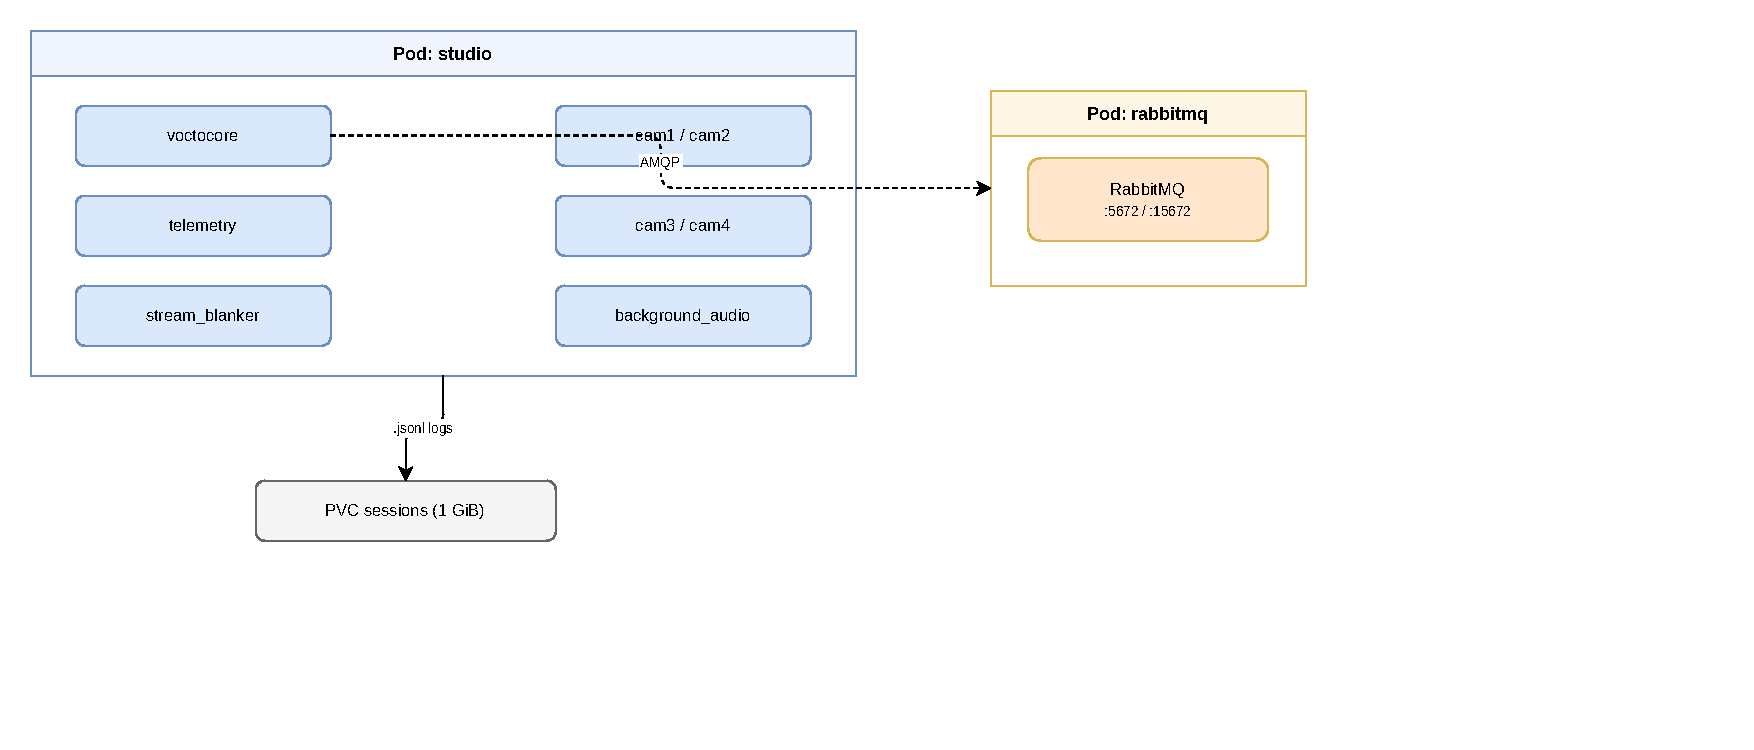
\includegraphics[width=\textwidth]{figuras/k8s_pods}
  \caption{Arquitectura de pods en el despliegue Kubernetes: el pod \texttt{studio}
           agrupa todos los contenedores del pipeline en un namespace de red compartido;
           \texttt{rabbitmq} corre como pod independiente; el PVC persiste los registros
           de sesión.}
  \label{fig:k8s_pods}
\end{figure}

\subsection{Sondas de preparación y orden de arranque}

La gestión de dependencias entre servicios se implementa en dos niveles:

\begin{itemize}
  \item \textbf{\texttt{initContainer} en studio:} antes de lanzar los contenedores
        principales, un \texttt{initContainer} basado en \texttt{busybox} ejecuta
        \texttt{until nc -zw1 rabbitmq 5672; do sleep 2; done}, bloqueando el arranque
        del pod hasta que RabbitMQ esté disponible en la red del clúster.
  \item \textbf{\textit{readinessProbe} de voctocore:} una sonda \texttt{tcpSocket}
        sobre el puerto 9999 con \texttt{initialDelaySeconds: 20} y
        \texttt{failureThreshold: 12} determina cuándo el núcleo está listo para
        aceptar conexiones, momento a partir del cual Kubernetes marca el pod como
        \textit{ready} y el tráfico puede enrutarse hacia él.
  \item \textbf{\textit{readinessProbe} de RabbitMQ:} ejecuta
        \texttt{rabbitmq-diagnostics ping} con reintentos cada 15~segundos, garantizando
        que el broker es funcional antes de que el servicio de telemetría intente
        publicar mensajes.
\end{itemize}

\subsection{Script de lanzamiento y port-forward}

El script \texttt{launch\_k8s.sh} unifica el ciclo de vida completo del clúster:
comprueba si Minikube y el pod de studio ya están en ejecución antes de lanzarlos
(evitando reinicios innecesarios), aplica los manifiestos con \texttt{kubectl apply},
espera a que todos los contenedores estén en estado \textit{ready} y establece un
\texttt{kubectl port-forward} que expone los puertos del pod
(9999, 9998, 11000, 12000, 14000--14005) en \texttt{localhost} del sistema anfitrión.
Esto permite que voctogui se conecte al clúster exactamente igual que en los escenarios
Docker o de dos PCs, sin modificar ningún parámetro de la interfaz gráfica.

La rutina \texttt{cleanup} registrada con \texttt{trap EXIT INT TERM} garantiza que
al cerrar voctogui se terminen el port-forward y los procesos de log asociados,
dejando el clúster en estado limpio y listo para un nuevo arranque inmediato.
